%begin preamble
\documentclass[12pt]{article} 
\setlength\parindent{0pt}

%packages
\usepackage{amsmath} % AMS Math Package
%\usepackage{siunitx} % si units
\usepackage{amssymb}	% Math symbols such as \mathbb
\usepackage{multicol} % Allows for multiple columns
\usepackage[small]{caption}%small captions
\usepackage{enumerate}%custom enumerations
\usepackage{enumitem} 
\usepackage{graphicx,epstopdf}
\usepackage{sectsty}
\usepackage{titlesec}
\usepackage[dvips,a4paper,top=1.54cm,bottom=3.25cm,left=3cm,right=3cm]{geometry}%margins and paper size
%end package

%cover page command
\newcommand{\makecover}[9]{
\thispagestyle{empty}
\setcounter{page}{0}
\begin{center}\LARGE{\bf #1}\vskip 24pt \normalsize{#2}\hspace*{\fill}\\
#3\vskip 12pt School of Physics and Astronomy\\The University of Manchester\vskip 12pt #4 Year MPhys Report\vskip 12pt
#5 \vskip 12pt
#6 \vskip 12pt
#7 \vskip 12pt
#8  \end{center}\section*{Abstract}

#9\newpage}

%end of coverpage command

\sectionfont{\normalsize\bfseries\fontfamily{ptm}\selectfont}
\subsectionfont{\normalsize\bfseries\fontfamily{ptm}\selectfont}
\subsubsectionfont{\normalsize\mdseries\fontfamily{ptm}\selectfont}

\pagestyle{plain}%page numbers in footer

%end preamble
\begin{document}

%Coverpage begin

%call \makecover with arguments: title, author, student id, year (first, second, third), date (mth year), partner name, abstract.
\makecover
{Discovering pulsars and transients with intelligent algorithms}
{Alex Lisboa-Wright}
{8928493}
{Fourth}
{January 2017}
{Project undertaken in collaboration with Lewis Smith (ID 8933715)}
{Project supervised by Dr Michael Keith}
{This is the first semester report of a full-year project}
{The aim of this project was to investigate whether using intelligent algorithms could lead to improvements in the classification of pulsars and transients. In this first semester, pulsars alone were studied, with special attention given to millisecond pulsars (MSPs). Various approaches were made in an attempt to improve classification. Adding realistic simulated MSP data to the HTRU2 dataset significantly improved the accuracy of the intelligent algorithms' classification of pulsars in general and MSPs as a subset. This was not replicated for the HTRU1 dataset, although this was probably due to the different processing pipelines used for the two datasets. Reducing the amount of noise data did cause a significant effect. Altering the period definition of MSPs did not significantly affect the accuracy for MSPs.}
%Coverpage end
\par
\section{Introduction}
\subsection{Pulsars and millisecond pulsars}
Pulsars are rapidly-rotating neutron stars formed during core-collapse supernovae (SNe). The gravitational pressure of the outer layers falling onto the core prior to the supernova event causes the core to contract rapidly and heat up, allowing the protons and electrons in the core to merge via inverse beta-decay to form neutrons and neutrinos. As the core contracts, conservation of angular momentum causes it to rotate much faster. As the neutrinos escape the core, a small fraction of them interact with the outer layers, transferring a huge quantity of energy which expels the layers violently - this is the supernova itself. If the core is below the Chandrasekhar mass limit of about 1.4 solar masses, neutron degeneracy pressure prevents it collapsing. The core is now a rapidly-rotating, extremely dense stellar remnant made of neutrons - a neutron star. Pulsars, detected by pulses of radiation aligned with the Earth's relative position, which emanate from the pulsar's magnetic poles (this is known as the lighthouse model) \cite{lorimer2008binary}, are characterized by a highly-stable period of rotation and pulse profile within each period, although there are significant differences between the profiles of different pulsars. While the pulsars do undergo a spin-down process due to loss of angular momentum over time, the rate of change in period is generally more than a dozen orders of magnitude less than the period itself for a given pulsar \cite{lorimer2008binary}, so even over the history of pulsar observation, the period can be treated as constant.
\paragraph{}
Millisecond pulsars (MSPs) are pulsars with a particularly high rotation frequency (low period), with the upper period limit for MSPs typically in the range of 10-30 milliseconds (ms). MSPs are of particular interest because their rotation rates are too high for isolated objects. Therefore, these pulsars are thought to undergo so-called ``spin-up" processes after the supernova event in which they were created \cite{lorimer2008binary}. Pulsars are of interest because of the extreme physics involve in their origins during SNe (the mechanism of which is not yet fully known) and their nature - they are testing grounds for general relativity and their interior structure is not yet understood.

\subsection{The High Time Resolution Universe (HTRU) Survey}
HTRU is a survey conducted, initially using the Parkes Radio Telescope in Australia for the southern hemisphere, and later, the Effelsberg Radio Telescope in Germany for the northern hemisphere additionally from 2010 onwards \cite{keith2010high}\cite{ng2012conducting}, with the purpose of scanning the entire plane of the sky for pulsar and transient signals at the highest resolution used so far in the field. It uses multi-beam receivers to increase the resolution and observes at a radio frequency of 1.4 GHz.
\paragraph{}
The survey's classification of raw data relies on the Stuttgart Neural Network Simulator (SNNS), an artificial neural net (ANN) created at the University of Stuttgart which uses 22 different features, including the period and dispersion measure as well as how the pulse profile shape matches to various curves, such as Gaussians \cite{thornton2013high}.

\subsection{Motivation}
The aim of this project is to improve the performance of machine learning (ML), or intelligent, algorithms on classification of pulsars in general and millisecond pulsars in particular, given their properties and the potential implications of those properties. Currently, candidate classification is carried out by processing the data into graphical form (see Figures \ref{psrsoftsim} and \ref{psrsoftnoise}), which can be analysed by eye as having characteristics of a pulsar \cite{morello2014spinn}. Pulsars can be determined by a relatively narrow and dark vertical region in the sub-band and sub-integration panels, a relatively compact single dark region in the period-DM plane, a profile histogram that forms something that is approximately a continuous curve and a single DM-SNR peak, since the pulsar is a single source. Therefore, the object in Figure \ref{psrsoftsim} is a good example of a pulsar, while the object in Figure \ref{psrsoftnoise} is clearly not. These images were generated using the psrsoft shell script \cite{thornton2013high}. For large quantities of data such as those from the upcoming Square Kilometre Array (SKA), this is time-consuming and consequently requires that the data be stored until it is analysed, which is infeasible for the rate of data production of surveys like the SKA. This motivates the main application of machine learning to radio astronomy, which is simultaneous recording and classification of data from large surveys such as the SKA. The ultimate objective of this is to separate data for potential astrophysical sources from the vast majority of received data, which is noise or radio frequency interference (RFI), which refers to Earth-based radio sources at observing frequencies, such as microwave ovens \cite{petroff2015identifying}, in real time. Using ML avoids the need to store impossibly large quantities of uninteresting data while, ideally, retaining all of the significant observations for further study using existing analysis techniques \cite{smits2009pulsar}.

\begin{figure}[h!]
\begin{center}
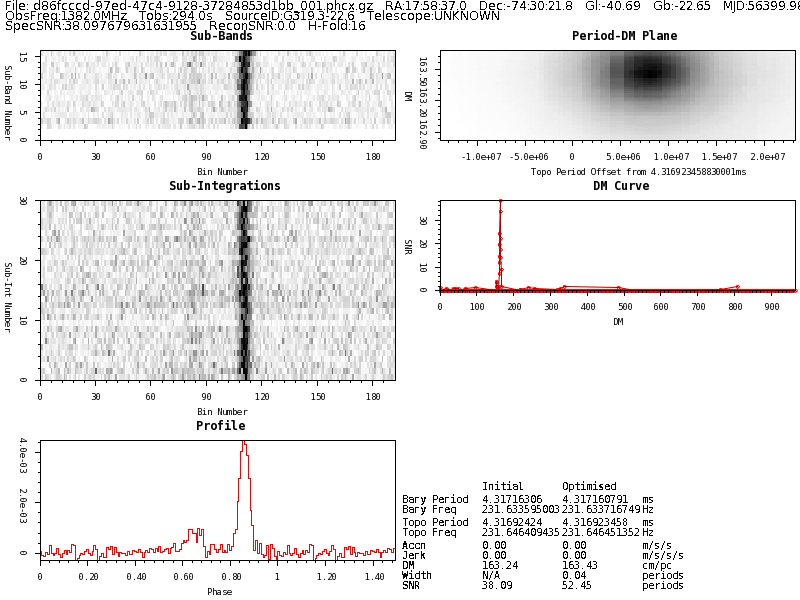
\includegraphics[scale=0.4]{d86fcccd-97ed-47c4-9128-37284853d1bb_001.png}
\caption{psrsoft image output for a simulated pulsar data file}
\label{psrsoftsim}
\end{center}
\end{figure}

\begin{figure}[h!]
\begin{center}
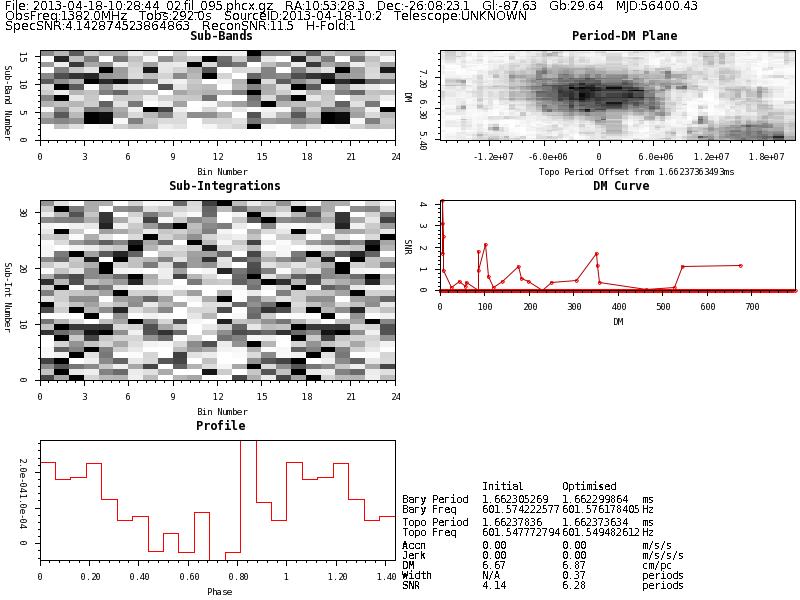
\includegraphics[scale=0.4]{2013-04-18-10_28_44_02_fil_095.png}
\caption{psrsoft image output for a non-pulsar (noise) data file}
\label{psrsoftnoise}
\end{center}
\end{figure}

\section{Machine learning}
\subsection{Theory}

Machine learning, as the name implies, is a process in which a computer is able to learn and adapt without detailed or specific additional programming being necessary. The mathematical objects which undergo machine learning are know as ``intelligent algorithms" for the same reason. Broadly speaking, there are 3 fundamental type of machine learning:

\begin{itemize}
\item Supervised learning: the algorithm (or ``classifier") is given a set of features (``inputs") to use for classifying data and a set of output classes (``targets") in which to place the data after the process, which are the only responses the algorithm can use.

\item Unsupervised learning: as before, the classifier is given the data and input features, but nothing else - the data is not divided by class at all, and the algorithm either ``memorises" the data to be recalled later, identifies underlying patterns in the data or tries to extract features from the data.

\item Reinforcement learning: the machine must adapt to a dynamic environment in order to best carry out its designated function. Examples include machines designed to play games autonomously.
\end{itemize}

Machine learning is applied to classify data by selecting and optimizing, or ``fitting", a mathematical model to the training dataset, in order to best separate the different classes by an $N$-dimensional hyperplane (where $N$ is the number of features used for classification) described by the model. During classification of the testing set, the model used on the set is produced by the training process. The nature of the model is important, and therefore the process of fitting it, and avoiding overfitting or underfitting it, is of paramount importance. An underfitted model (left-hand panel in Figure \ref{fitting}) is one which is too simple and could be more complicated while remaining applicable to different datasets (for example in cross-validation - see Section 2.1). An overfitted model (right-hand panel), by contrast, is specific to only one dataset - it adapts to separate the red and blue points almost perfectly in that dataset, but its accuracy is too sensitive to small changes in the data points, which will occur if it is applied to another dataset, thereby making the model virtually useless. An ideal model (centre panel) has some level of complexity to be able to separate the classes better than an underfitted model, but is equally accurate for different datasets.

\begin{figure}[h!]
\begin{center}
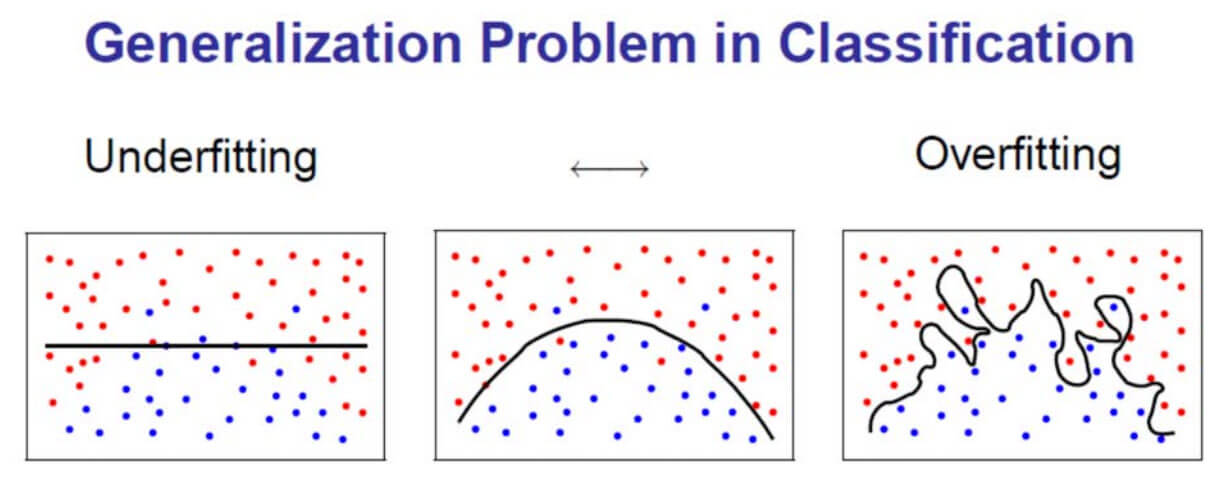
\includegraphics[scale=0.3]{overfitting.jpg}
\caption{Underfitting (left) and overfitting (right) of a classification model (solid black line) for the same dataset. Source: https://tomrobertshaw.net/2015/12/introduction-to-machine-learning-with-naive-bayes/}
\label{fitting}
\end{center}
\end{figure}

This project involved classifying datasets which distinguished between pulsar data points (referred to in this report on as ``class-1", ``positives" or ``pulsars") and non-pulsar data points (``class-0", ``negatives" or ``noise"). Since the objective of the classification in this case was to separate two pre-determined classes, it is an example of binary classification and supervised learning. During classification, two sets of data must be specified:
\begin{itemize}
\item The training set contains data used to optimize the model the algorithm uses.
\item The test set, on which the same model and algorithm are used to produce classification results.
\end{itemize}

The training process for large datasets often takes the form of $k$-fold cross-validation, or simply cross-validation. In this, the training dataset is divided into $k$ random subsets. One set is used to test the others against using the classification algorithm. The process is repeated $k$ times, and the average classification results are calculated and used to determine the measures of accuracy (see below) are calculated \cite{kohavi1995study}. The number of folds in cross-validation is important, as each subset needs to have enough variety within it to contribute meaningfully to the process - if it is too pure relative to the other subsets, the subset reacts differently towards the testing data subset in an adverse manner, which lowers the overall accuracy of the process. This is more likely to occur with a high $k$-value. If the $k$-value is too low, the cross-validation is not repeated enough times for the final average to be representative of the original dataset. Both cases cause the performance of the classification model produced by the cross-validation to deteriorate.

\subsection{Information theory}

To start classification, it is necessary to select features through which to express the original data. Determining the best set of features requires the use of information theory. For a given discrete random variable (in this case a data feature $X$), its information entropy, $H(X)$, is defined as a measure of the amount of information needed to describe the variable and the average information required to describe the variable \cite{bennasar2015feature}. It is defined as:

\begin{equation}
H(X)=-\sum_{x \in X}{P(x)\textrm{log}_{2}P(x)}
\end{equation}

where $P(x)$ is the probability of $x$ occurring (a.k.a. the probability mass function). From this equation, one can deduce that $0 \leqslant H(X) \leqslant 1$. The condition entropy, of a feature $X$ given another feature $Y$, is similarly defined as:

\begin{equation}
H(X|Y)=-\sum_{y \in Y}{P(y)\sum_{x \in X}{P(x|y)\textrm{log}_{2}P(x|y)}}
\end{equation}

where $P(y)$ is the probability of $y$ occurring and $P(x|y)$ is the probability of $x$ given $y$. The joint entropy of two variables $X$ and $Y$ is:

\begin{equation}
H(X,Y)=-\sum_{x \in X}\sum_{y \in Y}{P(x,y)\textrm{log}_{2}P(x,y)}
\end{equation}

where $P(x,y)$ is the joint probability of $x$ and $y$ \cite{bennasar2015feature}. In this project's datasets, the variable $Y$ takes the form of the class label \cite{lyon2016fifty}, which is the variable of most interest in this dataset, as it is the output variable in this project. The mutual information (MI), $I(X;Y)$, between $X$ and $Y$ is the amount of information that can be determined through one variable about another and can be defined in terms of their entropies by:

\begin{equation}
I(X;Y)= H(X) - H(X|Y)
\end{equation}

If two variables $X$ and $Y$ are statistically independent, their MI is zero. From this one can finally define the joint mutual information (JMI) of other features to a given feature $X$:

\begin{equation}
JMI(X)= \sum_{X' \in F} I(X,X';Y)
\end{equation}

where $F$ is the set of features other than $X$ \cite{lyon2016fifty} and $I(X,X';Y)$ is defined as \cite{bennasar2015feature}:
\begin{equation}
I(X,X';Y) = I(X;Y|X')+I(X';Y)
\end{equation}

\subsection{Classification measurements}

The results of binary classification come in the form of the true positive ($TP$), false positive ($FP$), true negative ($TN$) and false negative ($FN$) totals, which denote the number of each class (positive or negative) that were classified correctly or incorrectly, respectively, by the algorithm. These can be visualised concisely as the so-called confusion matrix \cite{kubat1998machine}, $C$, where:

\[
C =
  \begin{bmatrix}
    TP & FP \\
    FN & TN
  \end{bmatrix}
\]
These numbers are important in defining the following measures of accuracy \cite{lyon2016fifty}, which were used in this project. The recall, $R$, is the fraction of all true positives that were classified correctly:

\begin{equation}
R = \frac{TP}{TP + FN}
\label{recall}
\end{equation}

The precision, $P$, is the fraction of the classified positives which are actually positives:

\begin{equation}
P = \frac{TP}{TP + FP}
\label{prec}
\end{equation}

The specificity, $S$, is the negative analogue to the recall, as it is the fraction of true negatives that are correctly classified:

\begin{equation}
S = \frac{TN}{TN + FP}
\label{spec}
\end{equation}

The false positive rate, $FPR$, is equal to $1 - S$, as it is the fraction of negatives incorrectly classified as positives:

\begin{equation}
FPR = \frac{FP}{FP + TN}
\label{FPR}
\end{equation}

The geometric mean, or G-mean, $G$, is a measure which is sensitive to fractional misclassification, rather that the absolute value of the confusion elements themselves, \cite{kubat1998machine} and is defined as:

\begin{equation}
G = \sqrt{R \times S}
\label{gmean}
\end{equation}

Therefore, for datasets with a large imbalance in number between different class, such as the datasets used in this project, the G-mean is particularly sensitive to misclassification in the smaller class, in this case the pulsars. The F-score, $F$, is a measure that accounts for both precision and recall, and therefore is sensitive to overall fractional errors in the model for classifying positives:

\begin{equation}
F = 2 \times \frac{P \times R}{P+R}
\label{fscore}
\end{equation}

Finally, the overall accuracy, $A$, is the fraction of all of the data points which are correctly classified:

\begin{equation}
A = \frac{TP+TN}{TP+FP+TN+FN}
\label{accu}
\end{equation}

For datasets with a large imbalance between classes, such as datasets from pulsar surveys, which contain many more non-pulsars than pulsars, the accuracy became much less sensitive towards the algorithm's performance on the smaller class (pulsars in this example). This is problematic if, as in this project, the performance on the smaller class has more bearing on the final result. Therefore, the recall of the data was of greater interest than the accuracy for this project.

\subsection{Classifier algorithms}
The algorithms used in this project covered a wide range of properties and behaviours, since the aim of the project was to improve, and therefore prioritise, overall classifier performance in a general scenario, rather than focus on particular properties of certain algorithms. The ScikitLearn algorithm modules used \cite{scikit-learn} were:
\begin{itemize}
\item CART$\_$tree: Decision tree (DT) module. A decision tree separates data into different nodes depending on feature values, then splits the data within those nodes into more nodes and so on until the nodes contain data which best resembles the desired outputs. Small trees are easy to interpret visually as a series of logical steps (see Figure \ref{DTdiagram} in the Appendix) and trees in general are fast to construct compared to other types of logarithms, even for large datasets, and require little preparation of data. However, they are prone to overfitting and are often noisy \cite{friedman2001elements}.

\item Multi-layer Perceptron (MLP): An artificial neural net (ANN), which takes the set of features (see Figure \ref{MLPdiagram} in the Appendix, in the left-hand layer), known as the input layer, and generates the output layer (on the right) through one or more hidden layers in between. Each circle in Figure \ref{MLPdiagram} is called a neuron. Hidden layers each have an unknown number of neurons. Each neuron in a given layer connects to all neurons in the next layer with an individual weighting \cite{lisboa1993techniques}. The optimization is performed by reducing the errors when data points are passed along the connections. ANNs are less prone to overfitting than decision trees and can model more arbitrary functions to produce greater accuracy, but are generally slower.

\item NaiveBayes: Uses a simple approach in which the data features are assumed to be conditionally independent, given the class, and then applies Bayes' theorem to calculate the probability of each class given the features. \cite{john1995estimating}.

\item Support Vector Machine (SVM): Carries out a mapping in the $N$-dimensional feature space as described earlier, but is designed for datasets in which it is impossible to separate classes using a linear boundary to represent the model(``non-separable" data). It defines a non-linear boundary between classes by using a transformed version of the feature space, in which a linear boundary is created. The algorithm defines a band around the hyperplane, with a margin $M$ defined as the distance from the hyperplane to the limit of the band on either side \cite{friedman2001elements}. The perfect margin should have all points of one class on one side of it and all those of the other class on the other side. The points not in the correct regions have displacement vectors $\xi_{i}^{*}$ (see Figure \ref{svm}). The algorithm optimizes the model by maximising $M$ subject to a maximum value of the sum of all $\xi_{i}^{*}$.

\item Random$\_$Forest: An ensemble algorithm (which uses several individual algorithms) that compares a group of different decision trees to optimise the training set, through a prediction that averages the predictions of all trees, which are weighted individually, in the neighbourhood of a data point \cite{friedman2001elements}. Random forests are less susceptible to overfitting than individual trees.

\item AdaBoost: An ensemble algorithm which ``boosts", or improves, the performance of a group of classifiers, among which are some whose results are little better than random guesses, known as ``weak classifiers", by comparing the accuracy of each classifier to calculate a weight. The final predictive model is then a sum of the models of the individual classifiers multiplied by their individual weights. More accurate classifiers have a greater weight \cite{friedman2001elements}.
\end{itemize}

\begin{figure}[h!]
\begin{center}
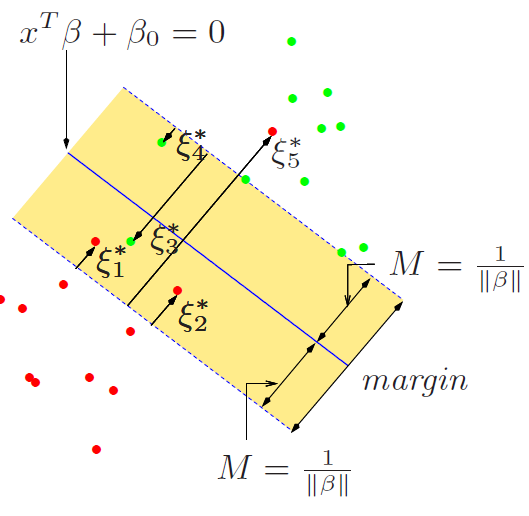
\includegraphics[scale=0.5]{svm.png}
\caption{SVM margin band (dashed line), with $\xi_{i}^{*}$ being the displacement vectors (in black) of each point from the correct region of the space. The model is the central blue line. Source: \cite{friedman2001elements}}
\label{svm}
\end{center}
\end{figure}

Additionally, the Gaussian-Hellenger Very Fast Decision Tree (GH-VFDT), as detailed by Lyon et al. \cite{lyon2016fifty}, was used to confirm the results of Table 11 in the same paper, but was then discarded.

\section{Experimental background - astrophysical measurements}
There are a number of important astrophysical measurements that are outputs of the telescope data. For instance, the average pulse profile is a graph of the average received amplitude as a function of the phase during an average pulse period. This profile is shown in the bottom left panel of Figures \ref{psrsoftsim} and \ref{psrsoftnoise} as a histogram. By comparing the panels of the two figures, it is clear that a signal from a pulsar will have a more obvious curve (in red) and a clear peak or peaks. Pilia et al. \cite{pilia2016wide}, using the LOw-Frequency ARray (LOFAR), demonstrate that there is a wide variety of pulse profile shapes, including multiple-peaked and heavily asymmetric profiles.
\paragraph{}
The signal-to-noise ratio (SNR) is simply the ratio, in a given reading, of the power from the source itself (the signal) versus that from other (background) objects, such as the cosmic microwave background (CMB), the atmosphere, the interstellar medium (ISM) or other origins (depending on the observing frequency), potentially including the telescope instrumentation itself. Readings with a higher SNR have a smaller relative error via signal averaging statistics, in which the SNR is proportional to the signal mean divided by the noise standard deviation, so are more likely to represent real source emission. The SNR can, however, be rendered less effective as a classification feature by RFI \cite{zhu2014searching}.
\paragraph{}
The dispersion measure (DM) is defined in terms of the electron number density, $n_{e}$, along the line of sight to the source \cite{ahuja2005tracking}:

\begin{equation}
DM = \int_{0}^{L}n_{e}dl
\label{dm}
\end{equation}

where $L$ is the line-of-sight distance to the source. The units of the DM are usually quoted as pc cm$^{-3}$, i.e., the DM can be interpreted as an electron column density along the line of sight. The DM is important because an ionized medium (such as the ISM) situated in between the observer and the source can cause the radiation from the source to become dispersed by refraction or absorption and re-radiation, depending on the wavelength of the incoming radiation. This causes a wavelength-dependent (and hence frequency-dependent) time delay in the reception of the signal. For two different frequencies, $f_{1}$ and $f_{2}$, the delay is given in SI units by:

\begin{equation}
\Delta t= \frac{e^2}{2\pi mc}(f_{1}^{-2} - f_{2}^{-2}) DM
\label{deltat}
\end{equation}

It is this frequency-dependent delay which is detected by the telescope's instrumentation, from which the DM is calculated. The DM can therefore be useful as a marker of the amount of gas between an observer and a given pulsar.

\section{Data and pipelines}
This project uses the data detailed by, and the PulsarFeatureLab processing pipeline created by, Lyon et al. \cite{lyon2016fifty}. PulsarFeatureLab was used to process the original and simulated data to extract the desired features. It is designed to be compatible with various data file formats and has multiple output file type options. In addition, its feature extractor program can output any of a selection of feature groups, and users can add their own feature list to this selection.

The datasets available for the chosen feature sets were labelled as follows:
\begin{itemize}
\item HTRU1: Dataset from HTRU processed by Morello et al. \cite{morello2014spinn}. Contained 74 classified MSPs, 1122 other classified pulsars and 89996 noise instances.
\item HTRU2: Dataset from HTRU processed by Lyon et al. \cite{lyon2016fifty} using PulsarFeatureLab. This was the principle test dataset in the first semester of the project. Contained 71 classified MSPs, 1568 other classified pulsars and 16259 noise instances.
\item LOTAAS: A dataset from the LOFAR Tied-Array All-Sky Survey (LOTAAS). This did not contain any classified MSPs and was therefore not useful for classification in this project.
\end{itemize}

In this project, MSPs and other pulsars (all treated during classification as being ``class 1") were distinguished by defining a threshold pulse period, below which classified pulsars were treated as MSPs and above which they were treated as non-MSPs. The definition described by Lorimer \cite{lorimer2008binary} of $P_{MSP}$ $\lesssim$ 30 ms was used as a guideline. The MSPs in the datasets, in order to include a few pulsars with periods slightly above 30ms, were defined as $P_{MSP}$ $\lesssim$ 31 ms. This was done to maximise the number of MSPs upon which to test the classifiers, although even with this there were relatively few MSPs in the datasets, as detailed above. For this project, the output files were chosen to be .arff (Attribute-Relation File Format) files in order to be compatible with the Waikato Environment Knowledge Analysis (WEKA) machine learning tool \cite{hall2009weka}, which was used to visualise and count the different data types and thus find potentially useful relationships between features to optimize simulated data.

\section{Experimental procedure}

The algorithms detailed in Table 11 of Lyon et al. \cite{lyon2016fifty} were run on all three datasets to test the reproducibility of the results. Then, with the exception of the GH-VFDT, those algorithms (or their ScikitLearn equivalents) were used as classifiers for the remainder of the experiment, together with the AdaBoost and RandomForest ensemble algorithms. To produce the best results, the data features had to be selected to give the best distinction between pulsars and non-pulsars while remaining easily processable. Feature selection was achieved using mutual information and then ranking features by their JMI score to list the best features and therefore select the better of the feature groups. Two groups were compared:

\begin{itemize}
\item Lyon features: Detailed by Lyon et al.\cite{lyon2016fifty}, this is a set of 8 features consisting of 4 statistical measures - the mean, standard deviation, skewness and kurtosis, which are the first, second, third and fourth statistical moments, respectively - applied to both the pulse profile and DM-SNR curve.
\item Thornton features: Detailed by Thornton \cite{thornton2013high}, this is the set of 22 features originally implemented for the SNNS (see Section 1.2).
\end{itemize}

The dataset judged to be better overall via averaging the JMI ranks of the features was used, together with the period, which was needed to separate the pulsars into MSPs and non-MSPs, and class values, which were designated as outputs, allowing for comparison of the cross-validation and test results with the real values.
\paragraph{}
To create the simulated pulsars, a programme called ``fake$\_$profiles.py" was created to simulate pulsars with a random distribution of SNRs greater than 5 and uniform distibution of periods in the range of 5-20 milliseconds. This period range was chosen in order to coincide with the expected area of interest for future MSP discoveries after consultation with the project supervisor. The simulated pulse profiles were injected into real noise data files to make the curves more realistic than using the simulated profiles alone, as these would be far too smooth and therefore too easy to distinguish from real data. To generate the final simulated data the injection was performed on a multiple-core GPU and left to run, due to the large processing power required. This produced directories each containing one simulated MSP data file and several noise files. The process used injection software provide by DSPSR \cite{van2011dspsr} and Tempo2 \cite{hobbs2006tempo2}.
\paragraph{}
To extract the pulsar file, a script called ``find$\_$fake$\_$pulsar.py" was created to allocate each file a score which was a sum of the fractional deviations of the pulse period and the DM value from the original injected data values. Therefore, the pulsar file would ideally have a score of zero. However, the fitting during the process allowed the parameters to be adjusted. The program compared the scores within each directory and took the lowest score forward. The relevant data file was then tested to determine whether its period and DM were within a strict tolerance level of the original injected values. The tolerance for the frequency/period was selected to be the maximum Doppler effect due to the orbital motion of the Earth, while the DM tolerance was set to be 0.7. Only if they passed this condition were they named as being the pulsar files, to ensure that the files which were produced were likely to be the correct ones. If no file met the requirements, a message to that effect was produced instead of a file name. The best simulation dataset was notable for the high proportion of pulsars found using this method. The feature data was extracted and converted into ARFF format using PulsarFeatureLab.
\paragraph{}
To check the suitability of the simulated data and look for relations between features, the data was manipulated to visualise the data in WEKA via plots such as Figures \ref{DMMeanStddevBadvsMSP} and \ref{DMMeanSkewBadvsMSPvsNon}. When the simulated data was declared viable for classification, a program named ``arff$\_$msp$\_$comment.py" was applied to the HTRU2 data, to add a comment to classified MSPs, allowing them to be distinguished from other real pulsars as well as the simulated MSPs. Using this comment, the real MSPs were removed from the HTRU2 data and placed into a separate ARFF file, which would be used as the testing dataset during classification.

\begin{figure}[h!]
\begin{center}
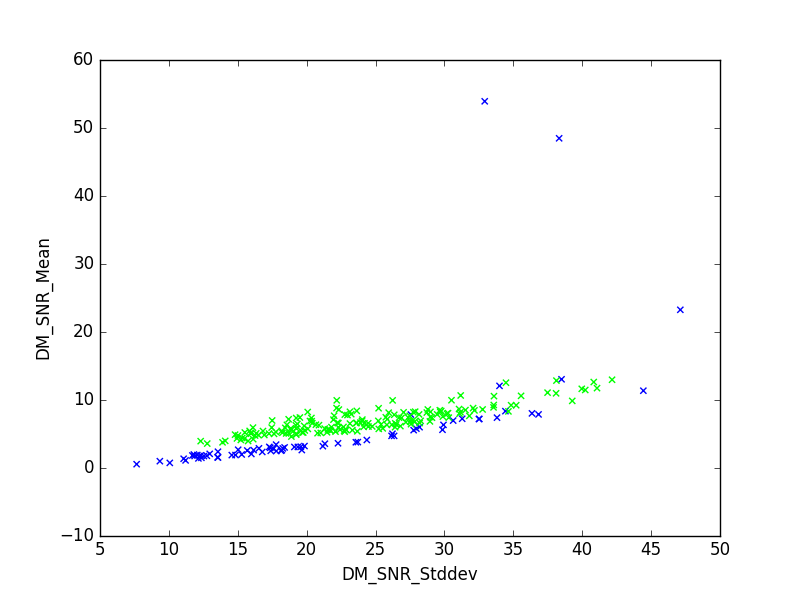
\includegraphics[scale=0.5]{htru2_msp(b)_sim_r3(g)_dm_mean_vs_stddev.png}
\caption{Unrealistic simulated MSP data (green) compared to HTRU2 MSPs (blue)}
\label{DMMeanStddevBadvsMSP}
\end{center}
\end{figure}

\begin{figure}[h!]
\begin{center}
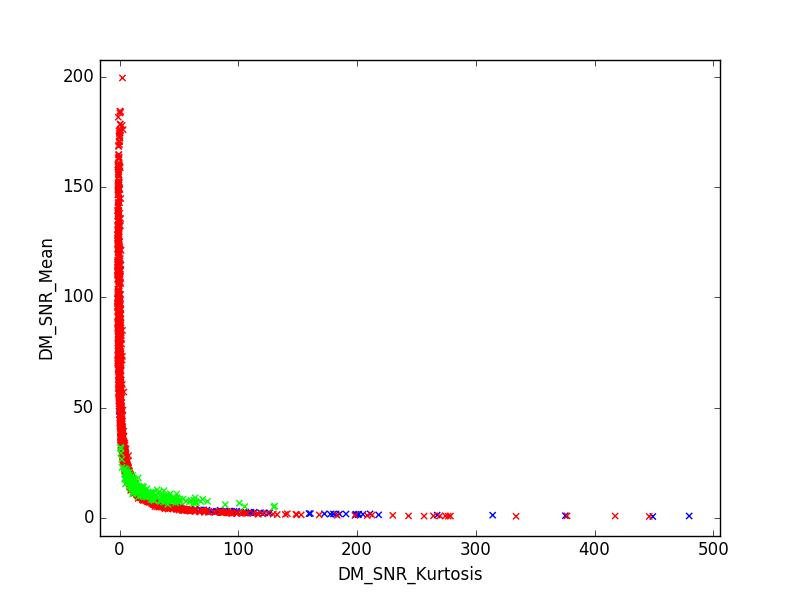
\includegraphics[scale=0.5]{htru2_msp(b)_non_msp(r)_sim_r3(g)_dm_mean_vs_skew.png}
\caption{Unrealistic simulated MSP data (green) compared to HTRU2 MSPs (blue) and non-MSPs (red)}
\label{DMMeanSkewBadvsMSPvsNon}
\end{center}
\end{figure}

\paragraph{}
The classification was carried out using ``evaluate$\_$classifier.py", which allowed the user to designate a training dataset for cross-validation, an optional testing set, the features to be used and the number of folds in the cross-validation, among other possible command line arguments. For classifying the real MSPs, the dataset containing everything except the real MSPs in each case was used for the training dataset and underwent cross-validation, with the non-MSP pulsars and simulated data (if applicable) being designated class-1 and the noise being class-0, with the number of folds set at $k$ = 5. During cross-validation, all of the classification measures detailed in Section 2.3 were displayed as outputs of the testing process to ensure that the cross-validation subsets were representative of the overall dataset - if any measure was abnormally high or low, the results were discarded and the program was run again, with any necessary adjustments to its input parameters being made in between runs. The real MSPs were then used as the testing set, using the model created by the cross-validation of the training data. Since the testing set was made up purely of class-1 objects (the real MSPs), the accuracy and recall of algorithms applied to that set are exactly the same by definition. This was done as part of the overall emphasis on the pulsars in the data.
\paragraph{}
A test of significance was carried out on the HTRU2 results generated before and after added the simulated MSPs to the training data, in the form of a student's t-test. A student's t-test was chosen as it controls for sample sizes, which is important, given the differences in pulsars numbers before and after adding the simulated MSPs. This generates a result, known as the p-value, using the two results and their respective standard deviations. This is then used to assess the validity, in this situation, of the null hypothesis \cite{friedman2001elements}, which states that any difference between two sets of results is purely due to random processes and thus the results are statistically equivalent. The threshold p-value was chosen as p$_{thres}$ = 0.05, which is a typical value and indicates that rejection of the null hypothesis is acceptable to a maximum error of 5$\%$ , with the p-value representing the actual calculated error. Hence, if the significance test generates a p-value less than p$_{thres}$, the null hypothesis is rejected and the difference between results is significant. If it generates a value greater than p$_{thres}$, the null hypothesis is accepted \cite{friedman2001elements}. Having used HTRU2 as a dataset to optimize the simulated data, the simulated data was added to HTRU1 and the algorithms were then applied to the resulting dataset.
\paragraph{}
As an extension, a program, ``plot$\_$classifier$\_$eval.py",  was written that would use the combined HTRU2 and simulated training dataset to determine the effect of varying the MSP cutoff period, $P_{MSP}$, on the MSP recall using the new definition. This was carried out by entering a quantity and range of $P_{MSP}$ values as arguments, then plotting the mean recalls against $P_{MSP}$, with error bars, for each classifier. The variation in definition was applied to real HTRU2 pulsars by adjusting the period threshold of ``arff$\_$msp$\_$comment.py" and applying it to HTRU2. This was carried out for both the newly-defined MSPs and all pulsars, as a reference. The results are shown in Figure \ref{allnoiseacc}.

\begin{figure}[h!]
\begin{center}
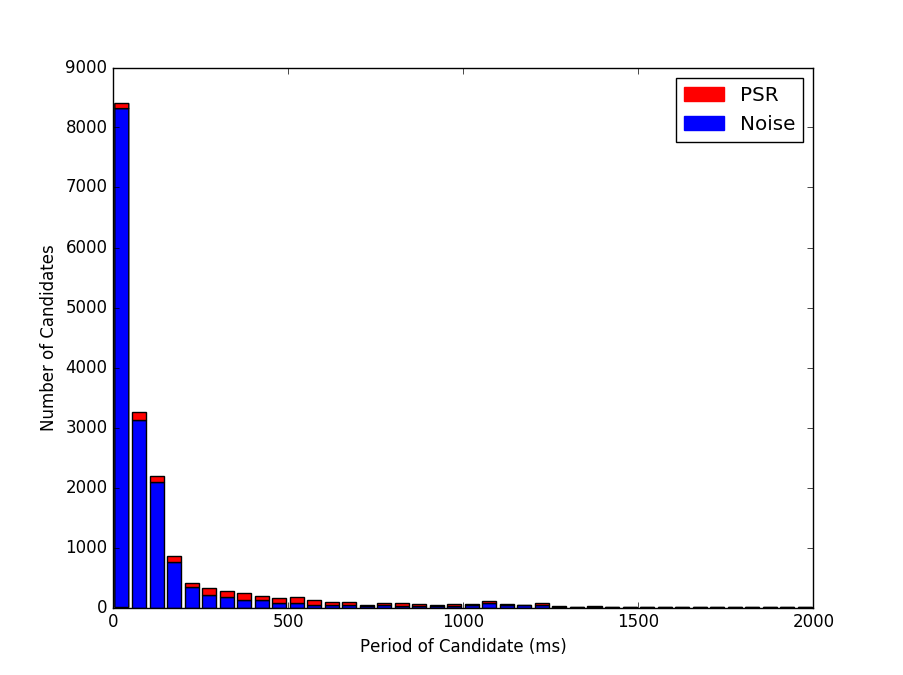
\includegraphics[scale=0.5]{htru2_period_hist.png}
\caption{Histogram of HTRU2 noise (blue) and pulsar (red) data, showing noise dominance, particularly at low periods}
\label{htru2hist}
\end{center}
\end{figure}

A final set of programs was written, allocating a random value between 0 and 1 to each noise data point with a period below $P_{MSP}$, setting a threshold and then separating the noise data according to that threshold. All files with values above the threshold were used as before in the training dataset for the classification. The rest were not used. This was done to investigate the effect of reducing the number of low-period noise data points on MSP recall, due to the overwhelming prior number dominance at low periods (see Figure \ref{htru2hist}). For the classification, the threshold was set at 0.9. For a noise sample as large as HTRU2, the distribution of random numbers would be more or less uniform, meaning that circa 90$\%$ of noise below $P_{MSP}$ was taken out of the classification process.

\section{Results}
The results detailed in Table 11 of Lyon et al. \cite{lyon2016fifty} were successfully reproduced, demonstrating their accuracy. After the mutual information values of every feature were calculated and the features were ranked by their respective JMI values, the Lyon features were found to be the more useful (see Table \ref{DTdiagram} in the Appendix).
\paragraph{}
When creating the simulated MSP data, the way in which the data was processed was very important with regard to how realistic it appeared in the feature space compared with real MSPs. Any datasets which had not been generated in the exact same way as the original HTRU2 data were easily distinguishable from the real data, particularly in their DM-SNR curve features. This is shown in Figure \ref{DMMeanStddevBadvsMSP}, where most simulated MSPs can clearly be separated from real MSPs by a line bisecting the lines followed by each group, and Figure \ref{DMMeanSkewBadvsMSPvsNon}, where the simulated MSPs do not follow the curve clearly traced by all the real pulsars. These differences adversely affect the model being used to classify real MSPs. The final simulated dataset, consisting of 744 simulated MSPs, did not deviate from the feature trends shown by the real pulsars upon visual inspection, and, within those trends, closely aligns with the regions occupied mostly by the real MSPs (see Figure \ref{htru2simr5} in the Appendix). Consequently, they were assessed to be realistic in the Lyon feature space.

\begin{table}[h!]
\centering
\resizebox{\columnwidth}{!}{%
\begin{tabular}{|l|l|l|l|}
\hline
\textbf{Classifier} & \textbf{$R$ for HTRU2 data} & \textbf{$R$ for HTRU2 + sim.} & \textbf{$R$ for reduced-noise HTRU2} \\ \hline
CART\_tree          & 0.301 $\pm$ 0.042                     & 0.594 $\pm$ 0.023               & 0.479 $\pm$ 0.064 \\ \hline
MLP                 & 0.383 $\pm$ 0.027                     & 0.603 $\pm$ 0.012               & 0.428 $\pm$ 0.016 \\ \hline
Naive\_Bayes        & 0.380 $\pm$ 0.000                     & 0.465 $\pm$ 0.000               & 0.372 $\pm$ 0.008 \\ \hline
SVM                 & 0.487 $\pm$ 0.013                     & 0.682 $\pm$ 0.008               & 0.490 $\pm$ 0.006 \\ \hline
Random\_Forest      & 0.293 $\pm$ 0.058                     & 0.563 $\pm$ 0.039               & 0.417 $\pm$ 0.068 \\ \hline
AdaBoost            & 0.358 $\pm$ 0.016                     & 0.558 $\pm$ 0.008               & 0.420 $\pm$ 0.027 \\ \hline
\end{tabular}
}
\caption{Recall on HTRU2 MSPs (class 1) using the HTRU2 noise (class 0) and non-MSPs (class 1) as training data}
\label{htru2}
\end{table}

\begin{table}[]
\centering
\begin{tabular}{|l|l|l|}
\hline
\textbf{Classifier} & \textbf{$R$ for HTRU1 data} & \textbf{$R$ for HTRU1 + simulated data} \\ \hline
CART\_tree          & 0.819 +/- 0.040                & 0.859 +/- 0.025                                 \\ \hline
MLP                 & 0.816 +/- 0.012                & 0.854 +/- 0.034                                 \\ \hline
Naive\_Bayes        & 0.811 +/- 0.000                & 0.824 +/- 0.000                                 \\ \hline
SVM                 & 0.981 +/- 0.007                & 0.986 +/- 0.000                                 \\ \hline
Random\_Forest      & 0.822 +/- 0.015                & 0.846 +/- 0.039                                 \\ \hline
AdaBoost            & 0.789 +/- 0.028                & 0.792 +/- 0.008                                 \\ \hline
\end{tabular}
\caption{Recall on HTRU1 MSPs (class 1) using the HTRU1 noise (class 0) and non-MSPs (class 1) as training data}
\label{htru2recall}
\end{table}

\begin{table}[]
\centering

\begin{tabular}{|l|l|l|}
\hline
\textbf{Classifier} & \textbf{p-value for HTRU2 data} & \textbf{p-value for HTRU1 data} \\ \hline
CART\_tree          & 0.000785                        & 0.267                           \\ \hline
MLP                 & 0.000372                        & 0.189                           \\ \hline
Naive\_Bayes        & 0.000230                        & 0.115                           \\ \hline
SVM                 & 3.94E-05                        & 0.340                           \\ \hline
Random\_Forest      & 0.00430                         & 0.273                           \\ \hline
AdaBoost            & 7.38E-05                        & 0.924                           \\ \hline
\end{tabular}
\caption{p-values from a student's t-test of significance for adding simulated data. The threshold p-value for both is 0.05.}
\label{htru2pvalue}
\end{table}

\begin{figure}[h!]
\begin{center}
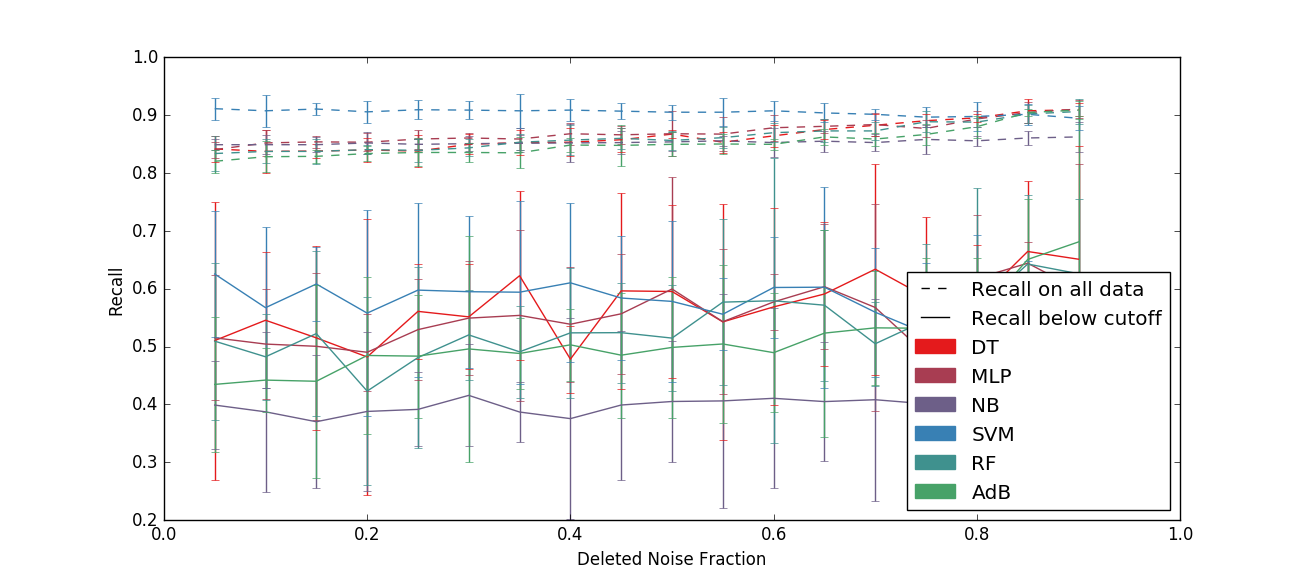
\includegraphics[scale=0.3]{acc_vs_noise_cutoff_all_noise.png}
\caption{Recall on MSPs as a function of the fraction of noise below $P_{MSP}$ which was removed from the data}
\label{allnoisecutacc}
\end{center}
\end{figure}

\begin{figure}[h!]
\begin{center}
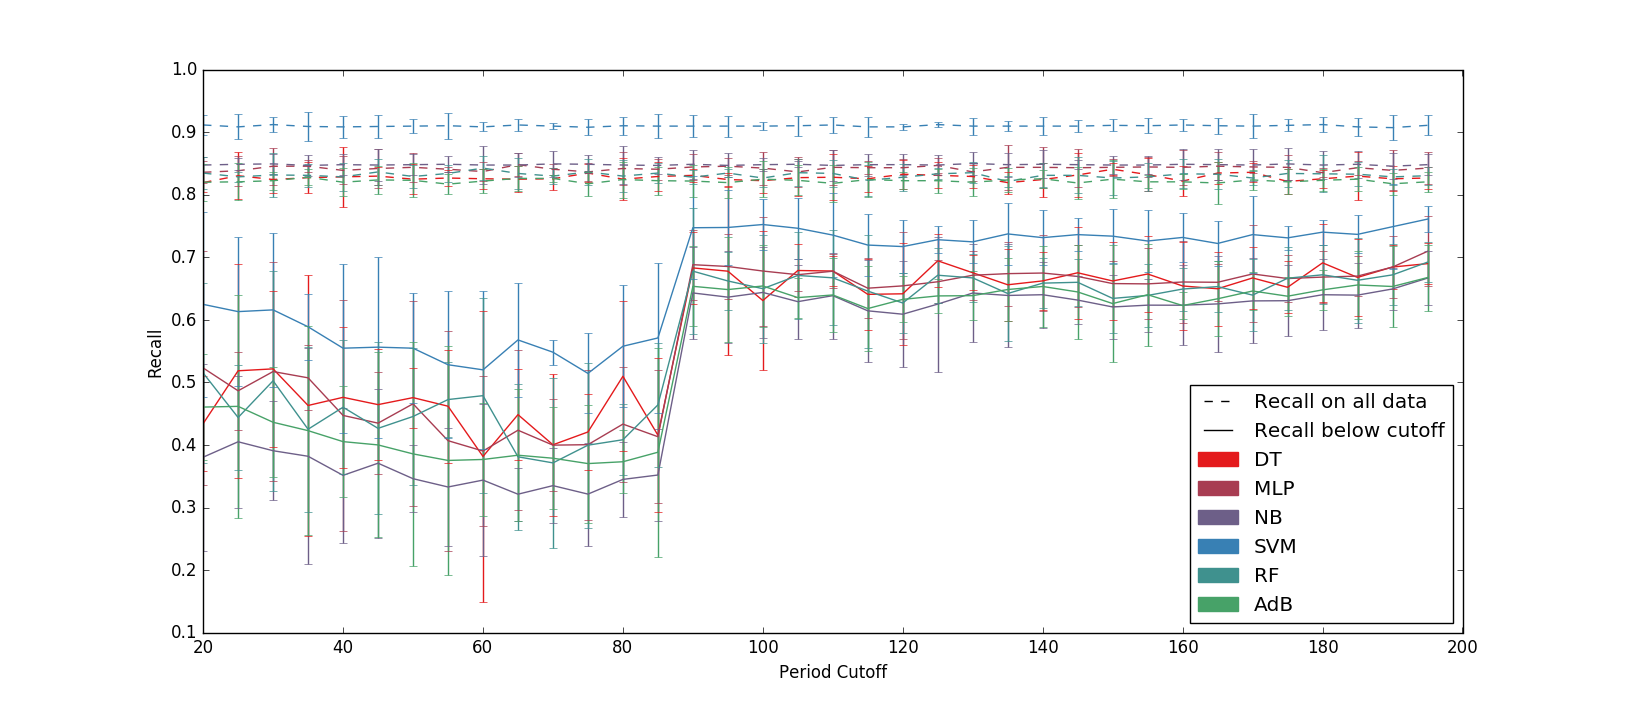
\includegraphics[scale=0.3]{acc_vs_period_v2_zoom.png}
\caption{Recall on MSPs for variation in the MSP cutoff period}
\label{allnoiseacc}
\end{center}
\end{figure}

\begin{figure}[h!]
\begin{center}
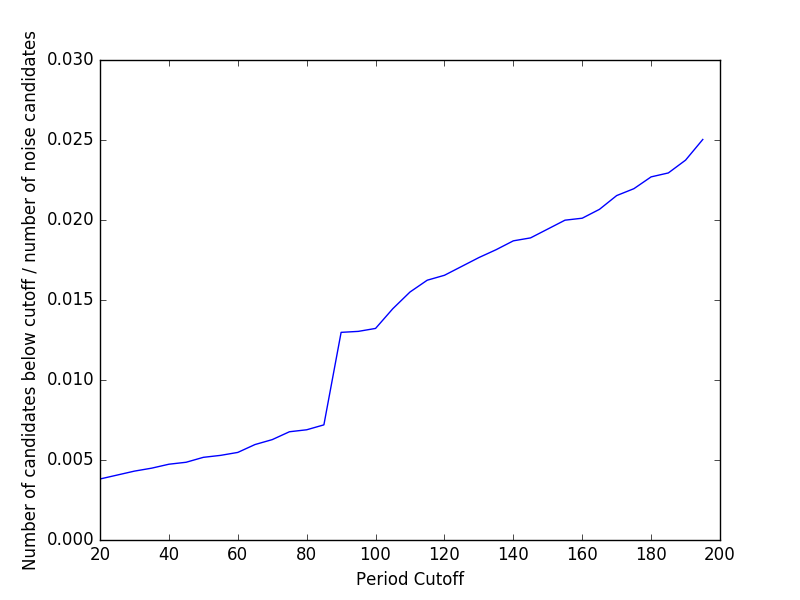
\includegraphics[scale=0.5]{noise_ratio_vs_period_cutoff_zoom.png}
\caption{Ratio of MSPs to noise candidates as a function of $P_{MSP}$}
\label{noiseratiocutoff}
\end{center}
\end{figure}

As shown in Figure \ref{allnoiseacc}, varying $P_{MSP}$, surprisingly, had no significant effect on the recall of MSPs, as can be seen via the errorbars. The SVM algorithm again proved to be the superior classifier, this time for all $P_{MSP}$. All classifiers appear to experience a sudden jump in recall between $P_{MSP}$ $\lesssim$ 80-100ms. Figure \ref{noiseratiocutoff} shows that, in the same interval, the ratio of labelled millisecond pulsars to noise files increases at a faster rate than for any other interval. Figure \ref{allnoisecutacc} shows that reducing the noise in the MSP period region has no significant effect on the MSP recall.

\section{Discussion}
The Lyon feature set is better for classifying pulsars by ML in this project partly because there are fewer features than is the case for the Lyon features, which makes the processing less complicated and quicker. Secondly, they are generic statistics-based features which directly relate to existing classification techniques, as they are simply the four lowest statistical moments of two of the graphics already used by human researchers to classify objects (see Figures \ref{psrsoftsim} and \ref{psrsoftnoise}). By contrast, some of the Thornton features are speculative, such as  $\chi^{2}$ results of fitting the pulse profile to various models, or are insensitive to some details, such as the feature using the area under the pulse profile, which can take the same value for a very narrow, tall profile or a broad, short profile, and which therefore requires additional features to extract the details, which is more inefficient. Thirdly, the speculative modelling features are only applicable to  pulsars, which must be known to have profiles which have a reasonable chance of matching the relevant models. For other objects, such as FRBs (to which we hope to extend the techniques used here on pulsars), modelling features may be less relevant. Also, the variety of pulse profiles shown by Pilia et al. \cite{pilia2016wide} indicates that speculative fittings may be even less efficient as features, since most will be redundant for any given pulsar and the pulsar may not conform adequately to any of them.
\paragraph{}
The addition of simulated data clearly and significantly improves the performance of the classification algorithms on the HTRU2 data. This is not only due to the realistic appearance of the data in the feature space, but also to the impact of adding a large number (744) of simulated MSPs to the real MSP population (71), as it counters the dominance of non-millisecond pulsars within the dataset of classified pulsars, as well as noise within the full dataset (see Section 4). The performance of the Naive$\_$Bayes classifier was the poorest of the classifiers overall and the standard deviation was sometimes so small as to be effectively zero, which is indicative of an underlying problem. This problem can be explained by the clear relationships between some of the features used - these relationships were, in fact, used to optimize the simulated data. As detailed in Section 2.4, the Naive$\_$Bayes classifier assumes the features it uses to be independent of one another, which is clearly contradicted by the aforementioned trends in the data. The performance of the SVM classifier was the best overall, which is likely due to its main strength of classifying non-separable data (see Section 2.4), of which the data in this project is an example (Figure \ref{htru2noisepsr} in the Appendix shows one part of the substantial mixing of data points from both classes in HTRU2, although the other datasets also displayed this property).
\paragraph{}
HTRU1 was not improved by any level of significance by the addition of the final simulated data. However, the classifiers performed very well without adding the simulated data, and adding it did not make the results worse - had the simulated data been unrealistic for HTRU1, it would have been expected that the results would have deteriorated. It must be noted, however, that HTRU1 and HTRU2 were processed using different pipelines methods and codes, which may explain how two sets of data from the same survey can produce such different performance levels from the same classifier algorithms and for every one of those algorithms. HTRU1 was processed using the PEASOUP pipeline, detailed by Morello et al. \cite{morello2014spinn}, while HTRU2 was processed using PDMP by Thornton \cite{thornton2013high}. The surprisingly high significance of how exactly a dataset was processed upon the data itself had already been witnessed when processing the simulated datasets (see Section 6). It could be that the HTRU1 data has been ``cleaned" to a greater extent than the HTRU2 data, hence the pulsar data points (most of which are for non-MSPs) are more easily classified correctly and it is difficult to introduce simulated MSP data which conforms to the same behaviour as the existing data.
\paragraph{}
The effect of varying the period threshold for defining MSPs is not significant, which is surprising, since MSPs are very clearly defined from an astrophysical perspective (see Section 1.1) as almost certainly being non-isolated objects, given the current understanding of pulsar mass constraints and the mechanism of angular momentum transfer in pulsar progenitor stars.  A sufficiently strict definition of MSPs should, in theory, allow the algorithms to focus exclusively on one area of feature space to find nearly all the MSPs, given the relations between features noted earlier for pulsars. The increase in recall in the 80-100 ms cutoff period interval is not significant for each classifier individually, but its transcendence of every algorithm in Figure \ref{allnoiseacc} suggests it is significant overall. However, the simultaneous increase in the MSP-to-noise candidate ratio in Figure \ref{noiseratiocutoff} suggests than the significance of the effect is due to the relatively rapid appearance of pulsar data points which are relatively easily classified correctly by all algorithms, as the period increases. This effect would not just be confined to the classification of these new data, since every point in Figure \ref{allnoiseacc} uses the whole HTRU2 dataset with the same classes. This means that with $P_{MSP}$ $\lesssim$ 80 ms, there are MSPs which have feature data values that are borderline for those MSP definitions, but fit relatively well with the new MSPs for $P_{MSP}$ $\gtrsim$ 80 ms, whose effect is to weight those regions of feature space such that the algorithms learn that potential pulsars in those regions are more likely to be real pulsars.
\paragraph{}
The effect of noise reduction is not significant, as shown in Figure \ref{allnoisecutacc} and Table \ref{htru2} if the relevant data and their standard deviations are considered. This suggests that correctly classifying pulsars will depend more on the pulsars themselves compared with how much RFI or noise data is gathered alongside them. Noise reduction is not particularly helpful with the applications of ML to pulsar detection (see Section 1.3), as it requires the data to be classified beforehand in order to reduce the noise and prevent the removal of real pulsar data, which requires data to be stored and then analysed closely.

\section{Conclusion}
For HTRU2, using only simulated MSPs or real non-MSPs as the class 1 objects in the training set produced low recall numbers on the real MSPs for all classifiers (see Table \ref{htru2}). In fact, the recall numbers were worse than if the class had been randomly guessed (which would have given $R \approx 0.5$). However, adding them both to the training data caused a highly significant increase in the recall for all of the (diverse) classifier algorithms. For HTRU1, this was not the case. However, using the real non-MSPs alone as the class 1 training data produced a high recall across all classifiers anyway, leaving little room for improvement after adding simulated MSPs. Doing so did not change the results significantly, not even detrimentally. Given the different behaviour of the same classifiers across all scenarios between the two datasets and given the fact that those sets were each processed by different groups using different computing pipelines, it is highly probable that the two facts are causally connected. For HTRU2, the recall on MSPs appears to be unaffected by both the position of $P_{MSP}$, which is surprising, and deleting most noise at low frequency.

\section{Direction for future work}
This project, as its title implies, is aimed at improving classification of both pulsars and transients such as fast radio bursts (FRBs). We hope to apply the techniques and experience gained with pulsars during this semester to FRBs next semester. Given the rarity of FRBs (less than 20 confirmed as of the sart of 2017, including 1 repeating source \cite{scholz2016repeating}) and the substantial similarity between their signals and terrestrial sources, particularly swept-frequency terrestrial transient signals known as ``perytons" \cite{petroff2015identifying}, it will require fine-tuning. The features used will have to be evaluated again - the Lyon features would appear to be a favourable starting point due to their statistical nature, which could allow these features to be more easily generalised to non-pulsar target data. However, this is not guaranteed.

\begin{small}
\bibliographystyle{ieeetr}
\bibliography{mphysref1}
\end{small}

\section{Appendix}
\subsection{Source code repository}
https://github.com/lsgos/MPhysPulsars

Contains source code, datasets, simulated data, results in .png, .ods and .txt formats and a copy of PulsarFeatureLab. All new codes for this computer-based project were written in Python 2.7.12.

\subsection{Risk assessment}
\underline{1. Hazard identification:}
\begin{enumerate}[label=(\roman*)]
\item High computer usage and the subsequent risk of sight problems due to overexposure to screens.
\item Electrocution
\end{enumerate}
\underline{2. People at risk:}
\begin{enumerate}[label=(\roman*)]
\item MPhys participants
\item MPhys participants
\end{enumerate}
\underline{3. Risk evaluation:}
\begin{enumerate}[label=(\roman*)]
\item The risk is adequately controlled due to industry standards and user guidance regarding computer screen usage.
\item The risk is adequately controlled due to grounding and insulation of wires.
\end{enumerate}
\underline{4. Actions to be taken:}
\begin{enumerate}[label=(\roman*)]
\item Take regular breaks away from computer screens.
\item Follow standard guidelines for use of electrical equipment.
\end{enumerate}
Last reviewed: 15th December 2016 \newline
Carried out by: Alex Lisboa-Wright, Lewis Smith.

Supervisor: Michael Keith.

\subsection{Additional tables and figures}
\begin{table}[]
\centering
\resizebox{\columnwidth}{!}{%
\begin{tabular}{|l|l|l|}
\hline
\textbf{Feature}                                    & \textbf{Average mutual info} & \textbf{Average JMI rank} \\\hline
\textbf{Profile Kurtosis (Lyon)}                                & 0.157            & 1.33          \\
Best SNR                                            & 0.135            & 3.33          \\
Pulse Width                                         & 0.139            & 4.33          \\
\textbf{Profile Mean (Lyon)}                                 & 0.139            & 4.67 \\
$\chi ^{2}$ of pulse profile and sine$^{2}$         & 0.122            & 9                         \\
Number of profile peaks                             & 0.0679              & 9                         \\
Best DM                                             & 0.117             & 10                        \\
$\chi ^{2}$ of pulse profile and double Gaussian    & 0.114             & 10                        \\
Area under profile after mean subtraction           & 0.0936              & 10.3          \\
\textbf{Profile skewness (Lyon)}                             & 0.127              & 10.7          \\
\textbf{DM kurtosis (Lyon)}                                  & 0.0832            & 11.3 \\
Best Period                                         & 0.116            & 11.3          \\
Offset of profile histogram from zero               & 0.117           & 14.3          \\
Thornton feature 15                                 & 0.0152           & 15.3          \\
\textbf{Profile standard deviation (Lyon)}                   & 0.0609            & 16                        \\
\textbf{DM skewness (Lyon)}                                  & 0.0328              & 16.3          \\
\textbf{DM mean (Lyon)}                                      & 0.0499            & 17.3 \\
average of corrolation coefficient in sub-bands     & 0.0243              & 18.3          \\
\textbf{DM standard deviation (Lyon)}                        & 0.0603            & 18.7          \\
abs(DM$\_${fit} $-$ DM$\_$best)                     & 0.0284            & 18.7          \\
$\chi ^{2}$ of DM-SNR fit                           & 0.0251              & 18.7          \\
Offset of Thornton feature 11 and profile gradient histogram & 0.0281            & 19                     \\
max(profile) / max(fitted Gaussian)                 & 0.0293              & 19.3          \\
sum of correlation coefficient in sub-bands         & 0.0108             & 20                        \\
Thornton feature 14                                 & 0.0134             & 20.7          \\
FWHM of Gaussian                                    & 0.00321            & 25                        \\
RMS of peak position in sub-bands                   & 0.000306           & 27.3          \\
mean FWHM of double Gaussian                        & 7.78E-05         & 27.7          \\
$\chi ^{2}$ of pulse profile and sine               & 4.27E-05         & 28.3          \\
$\chi ^{2}$ of pulse profile and Gaussian           & 3.33E-05         & 28.7         \\\hline
\end{tabular}
}
\caption{Mutual information values and JMI ranks averaged over all 3 datasets. Lyon features \cite{lyon2016fifty} are marked in bold. All others are Thornton features \cite{thornton2013high}.}
\label{avgJMI}
\end{table}

\begin{figure}[h!]
\begin{center}
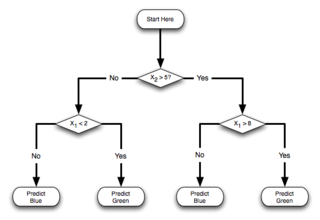
\includegraphics[scale=0.7]{DecisionTree_Classification_Graphic_small.png}
\caption{Diagram of a decision tree for color prediction. Source: https://alliance.seas.upenn.edu/~cis520/wiki/index.php?n=Lectures.DecisionTrees}
\label{DTdiagram}
\end{center}
\end{figure}

\begin{figure}[h!]
\begin{center}
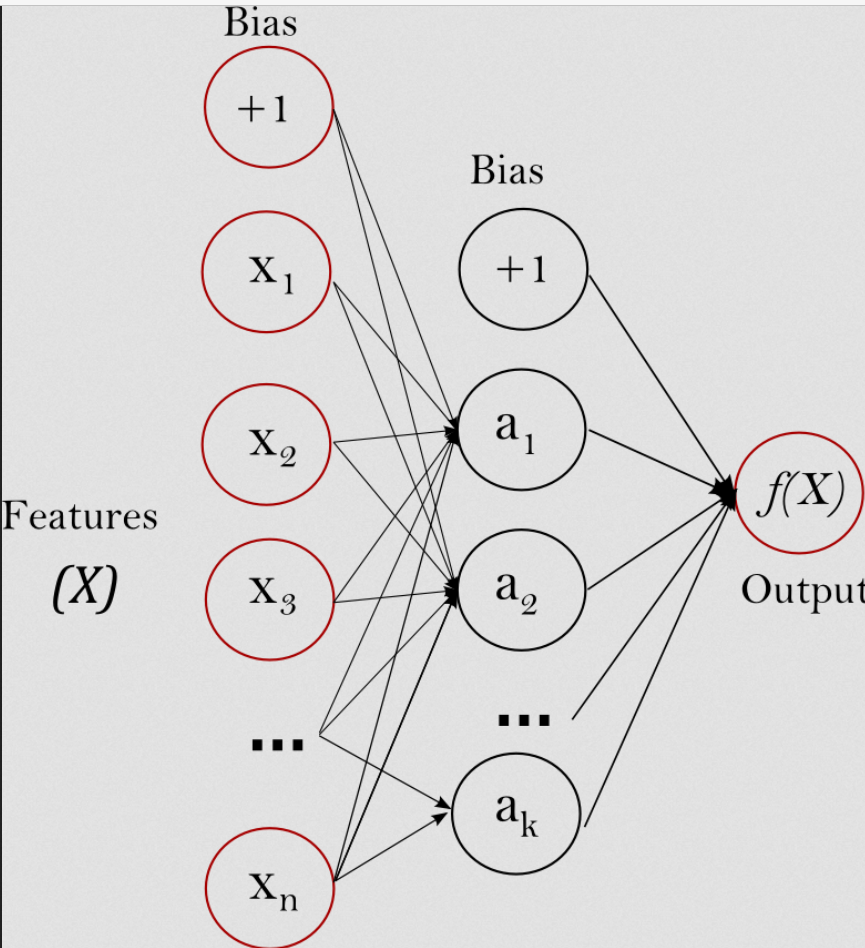
\includegraphics[scale=0.3]{multilayerperceptron_network.png}
\caption{Diagram of an ANN (specifically the MLP) with one hidden layer. Source: http://scikit-learn.org/stable/modules/neural$\_$networks$\_$supervised.html}
\label{MLPdiagram}
\end{center}
\end{figure}

\begin{figure}[h!]
\begin{center}
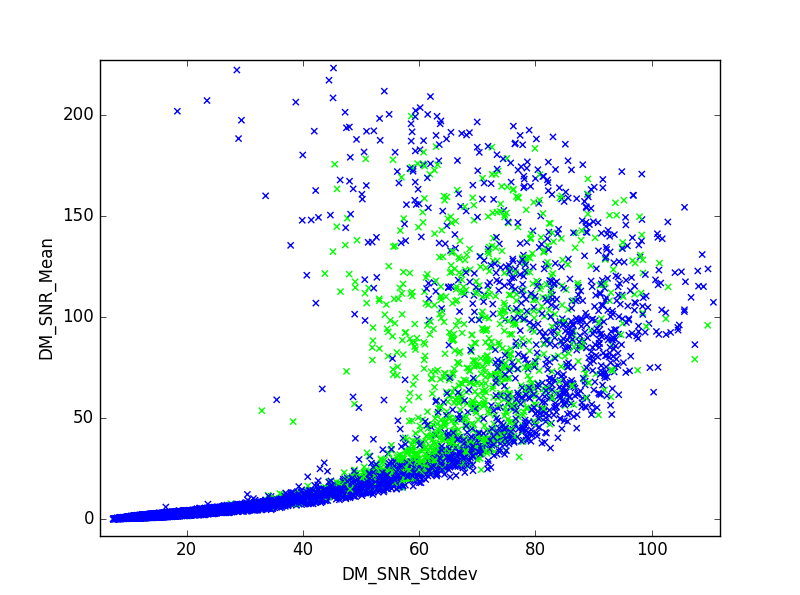
\includegraphics[scale=0.5]{htru2_noise(b)_psr(g)_dm_mean_vs_stddev.png}
\caption{Raw HTRU2 data: pulsars (green), including MSPs, compared to noise (blue)}
\label{htru2noisepsr}
\end{center}
\end{figure}

\begin{figure}[h!]
\begin{center}
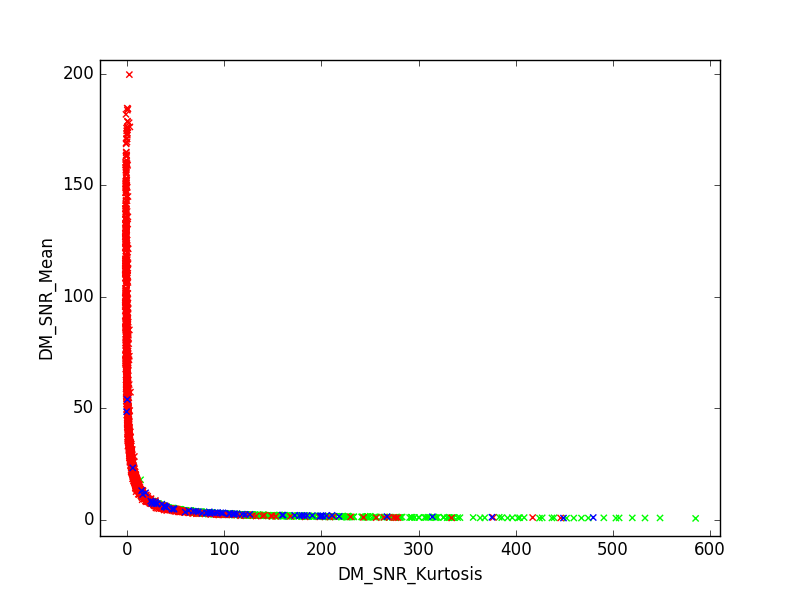
\includegraphics[scale=0.5]{htru2_msp(b)_non_msp(r)_sim_r5(g)_dm_mean_vs_skew.png}
\caption{Final (realistic) simulated MSP data (green) compared to HTRU2 MSPs (blue) and non-MSPs (red)}
\label{htru2simr5}
\end{center}
\end{figure}

\end{document}